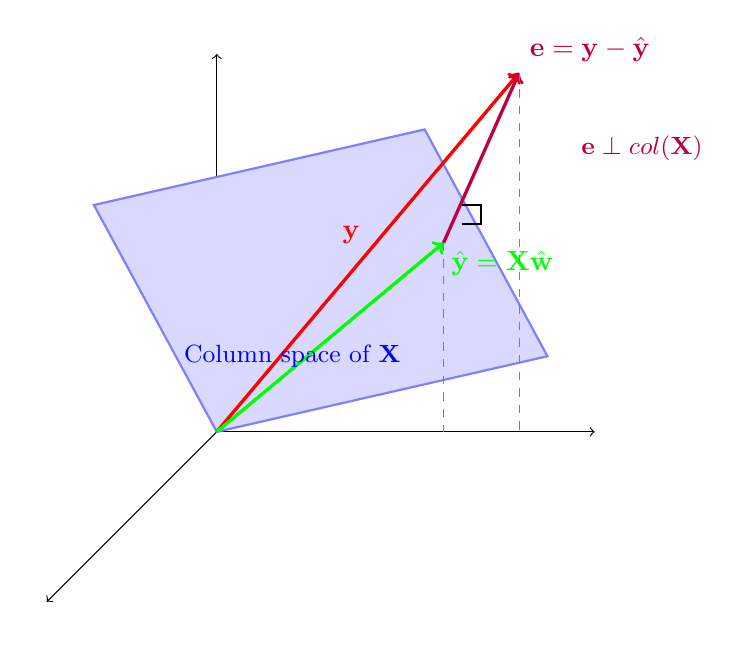
\begin{tikzpicture}[scale=1.2]
  % 3D-like coordinate system
  \draw[->] (0,0) -- (4,0) node[right] {};
  \draw[->] (0,0) -- (0,4) node[above] {};
  \draw[->] (0,0) -- (-1.8,-1.8) node[below left] {};
  
  % Column space (more 3D-like plane)
  \fill[blue!15] (0,0) -- (3.5,0.8) -- (2.2,3.2) -- (-1.3,2.4) -- cycle;
  \draw[thick, blue!50] (0,0) -- (3.5,0.8) -- (2.2,3.2) -- (-1.3,2.4) -- cycle;
  
  % Target vector y (outside column space) - more prominent
  \draw[very thick, red, ->] (0,0) -- (3.2,3.8) node[midway, above left=-1pt] {$\mathbf{y}$};

  % Projection onto column space - more prominent
  \draw[very thick, green, ->] (0,0) -- (2.4,2.0) node[below right=-1pt] {$\hat{\mathbf{y}} = \mathbf{X}\hat{\mathbf{w}}$};
  
  % Residual vector (orthogonal) - more prominent
  \draw[very thick, purple, ->] (2.4,2.0) -- (3.2,3.8) node[above right] {$\mathbf{e} = \mathbf{y} - \hat{\mathbf{y}}$};
  
  % Clearer orthogonality symbol
  \draw[thick] (2.6, 2.2) -- (2.8, 2.2) -- (2.8, 2.4) -- (2.6, 2.4);
  
  % Additional annotations
  \draw[dashed, gray] (2.4, 2.0) -- (2.4, 0);
  \draw[dashed, gray] (3.2, 3.8) -- (3.2, 0);
  
  % Labels (no internal title: the book's figure caption carries it)
  \node[blue, font=\small] at (0.8, 0.8) {Column space of $\mathbf{X}$};
  \node[purple, font=\small] at (4.5, 3.0) {$\mathbf{e} \perp \text{col}(\mathbf{X})$};
\end{tikzpicture}
